% --- Fix fuer Scholze 10.tex ---
% In die Praeambel aufnehmen (vor \begin{document})
\usepackage{amsthm}

% Falls noch nicht vorhanden:
\theoremstyle{plain}
\newtheorem{satz}{Satz}[section]
\newtheorem{lemma}[satz]{Lemma}
\newtheorem{proposition}[satz]{Proposition}
\newtheorem{korollar}[satz]{Korollar}

\theoremstyle{definition}
\newtheorem{definition}[satz]{Definition}
\newtheorem{bemerkung}[satz]{Bemerkung}
\newtheorem{beispiel}[satz]{Beispiel}
\newtheorem{remark}[satz]{Remark} % falls im Text weiterhin englisch \begin{remark} benutzt wird

% Wenn du durchgehend deutsch willst, ersetze im Text stattdessen
% \begin{remark} ... \end{remark}
% durch
% \begin{bemerkung} ... \end{bemerkung}

% --- Grafische Ergaenzung mit pgfplots ---
% Ebenfalls in die Praeambel:
\usepackage{pgfplots}
\pgfplotsset{compat=1.18}

% --- Beispielsection fuer den Hauptteil ---
\section{Grafische Erg\"anzung: renormierte Geschwindigkeiten und Hurwitzdruck}

Abbildung~\ref{fig:hurwitz-speeds} visualisiert die renormierten Geschwindigkeiten
\(\tilde c_t^{(N)}\), \(\tilde c_e^{(N)}\) sowie den renormierten Hurwitzdruck
\(\widehat D_H^{(N)}=\tilde c_e^{(N)}-\tilde c_t^{(N)}\) f\"ur die Pilotwerte
\(N=20,33,50,100,137,200,500,1000,2000,5000\).

\begin{figure}[htbp]
    \centering
    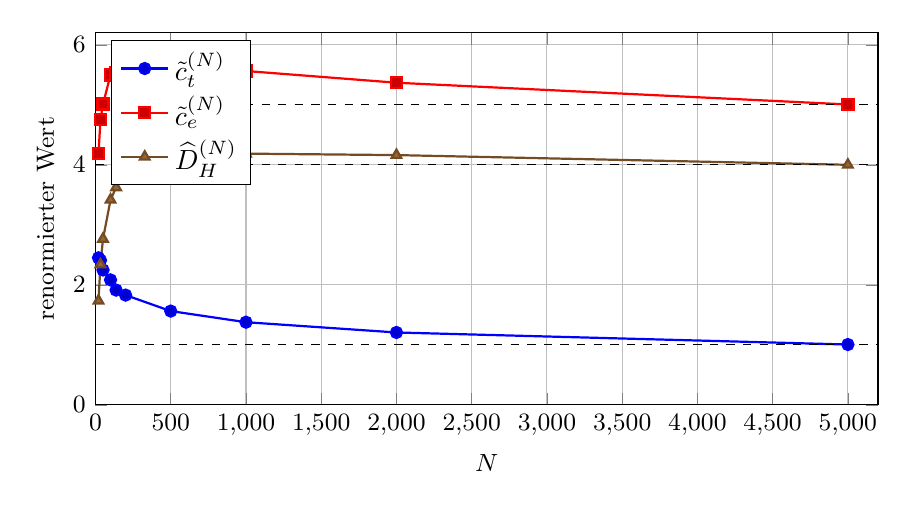
\begin{tikzpicture}
    \begin{axis}[
        width=0.95\textwidth,
        height=0.52\textwidth,
        xlabel={$N$},
        ylabel={renormierter Wert},
        xmin=0, xmax=5200,
        ymin=0, ymax=6.2,
        grid=both,
        legend style={at={(0.02,0.98)},anchor=north west,fill=white},
        tick label style={font=\small},
        label style={font=\small},
        legend cell align=left,
    ]

    % ct
    \addplot+[mark=*, thick] coordinates {
        (20,2.45067)
        (33,2.40957)
        (50,2.24815)
        (100,2.08298)
        (137,1.91296)
        (200,1.82946)
        (500,1.56305)
        (1000,1.37771)
        (2000,1.20647)
        (5000,1.00555)
    };
    \addlegendentry{$\tilde c_t^{(N)}$}

    % ce
    \addplot+[mark=square*, thick] coordinates {
        (20,4.18535)
        (33,4.75084)
        (50,5.01468)
        (100,5.50069)
        (137,5.53736)
        (200,5.67169)
        (500,5.67858)
        (1000,5.56530)
        (2000,5.36985)
        (5000,5.00720)
    };
    \addlegendentry{$\tilde c_e^{(N)}$}

    % DH hat
    \addplot+[mark=triangle*, thick] coordinates {
        (20,1.73468)
        (33,2.34127)
        (50,2.76652)
        (100,3.41771)
        (137,3.62440)
        (200,3.84221)
        (500,4.11547)
        (1000,4.18770)
        (2000,4.16335)
        (5000,4.00149)
    };
    \addlegendentry{$\widehat D_H^{(N)}$}

    % Referenzlinien
    \addplot[dashed, domain=0:5200, samples=2] {1};
    \addplot[dashed, domain=0:5200, samples=2] {4};
    \addplot[dashed, domain=0:5200, samples=2] {5};

    \end{axis}
    \end{tikzpicture}
    \caption{Renormierte topologische Geschwindigkeit \(\tilde c_t^{(N)}\), renormierte elektrodynamische Geschwindigkeit \(\tilde c_e^{(N)}\) und renormierter Hurwitzdruck \(\widehat D_H^{(N)}\). Die gestrichelten Linien bei $1$, $4$ und $5$ markieren die vermuteten asymptotischen Niveaus.}
    \label{fig:hurwitz-speeds}
\end{figure}

% --- Optional: zweite Grafik fuer zeta-modulierte Werte (M=137) ---
\section{Grafische Erg\"anzung: zeta-modulierte effektive Geschwindigkeiten}

\begin{figure}[htbp]
    \centering
    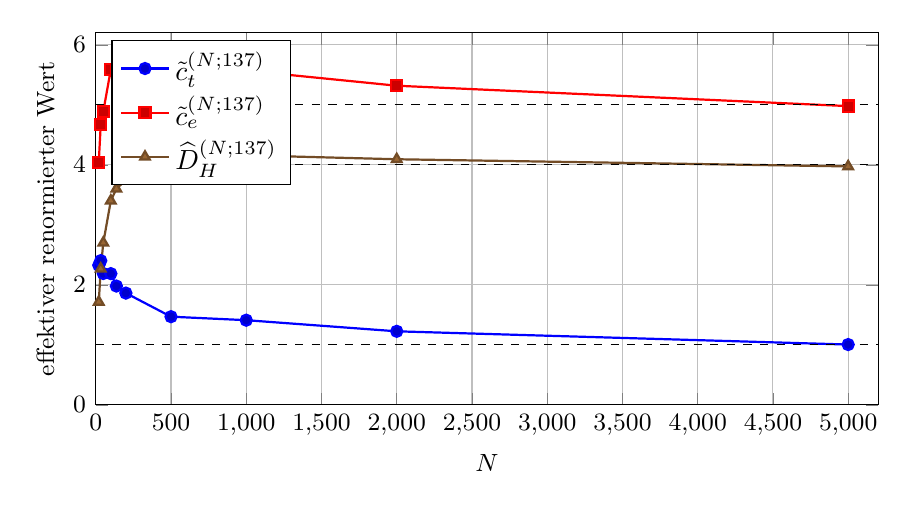
\begin{tikzpicture}
    \begin{axis}[
        width=0.95\textwidth,
        height=0.52\textwidth,
        xlabel={$N$},
        ylabel={effektiver renormierter Wert},
        xmin=0, xmax=5200,
        ymin=0, ymax=6.2,
        grid=both,
        legend style={at={(0.02,0.98)},anchor=north west,fill=white},
        tick label style={font=\small},
        label style={font=\small},
        legend cell align=left,
    ]

    \addplot+[mark=*, thick] coordinates {
        (20,2.327592)
        (33,2.404055)
        (50,2.189332)
        (100,2.187470)
        (137,1.980480)
        (200,1.862981)
        (500,1.469579)
        (1000,1.411328)
        (2000,1.225873)
        (5000,1.005182)
    };
    \addlegendentry{$\tilde c_t^{(N;137)}$}

    \addplot+[mark=square*, thick] coordinates {
        (20,4.044098)
        (33,4.672809)
        (50,4.891004)
        (100,5.590390)
        (137,5.582091)
        (200,5.611208)
        (500,5.571141)
        (1000,5.571147)
        (2000,5.319948)
        (5000,4.979917)
    };
    \addlegendentry{$\tilde c_e^{(N;137)}$}

    \addplot+[mark=triangle*, thick] coordinates {
        (20,1.716506)
        (33,2.268754)
        (50,2.701672)
        (100,3.402919)
        (137,3.601611)
        (200,3.748226)
        (500,4.101562)
        (1000,4.159819)
        (2000,4.094075)
        (5000,3.974735)
    };
    \addlegendentry{$\widehat D_H^{(N;137)}$}

    \addplot[dashed, domain=0:5200, samples=2] {1};
    \addplot[dashed, domain=0:5200, samples=2] {4};
    \addplot[dashed, domain=0:5200, samples=2] {5};

    \end{axis}
    \end{tikzpicture}
    \caption{Zeta-modulierte effektive Geschwindigkeiten und zeta-modulierter renormierter Hurwitzdruck f\"ur $M=137$ Nullstellen.}
    \label{fig:hurwitz-speeds-zeta}
\end{figure}
